\section{Silicon Tungsten SiD ECAL}
\subsection{Introduction}
\begin{figure}
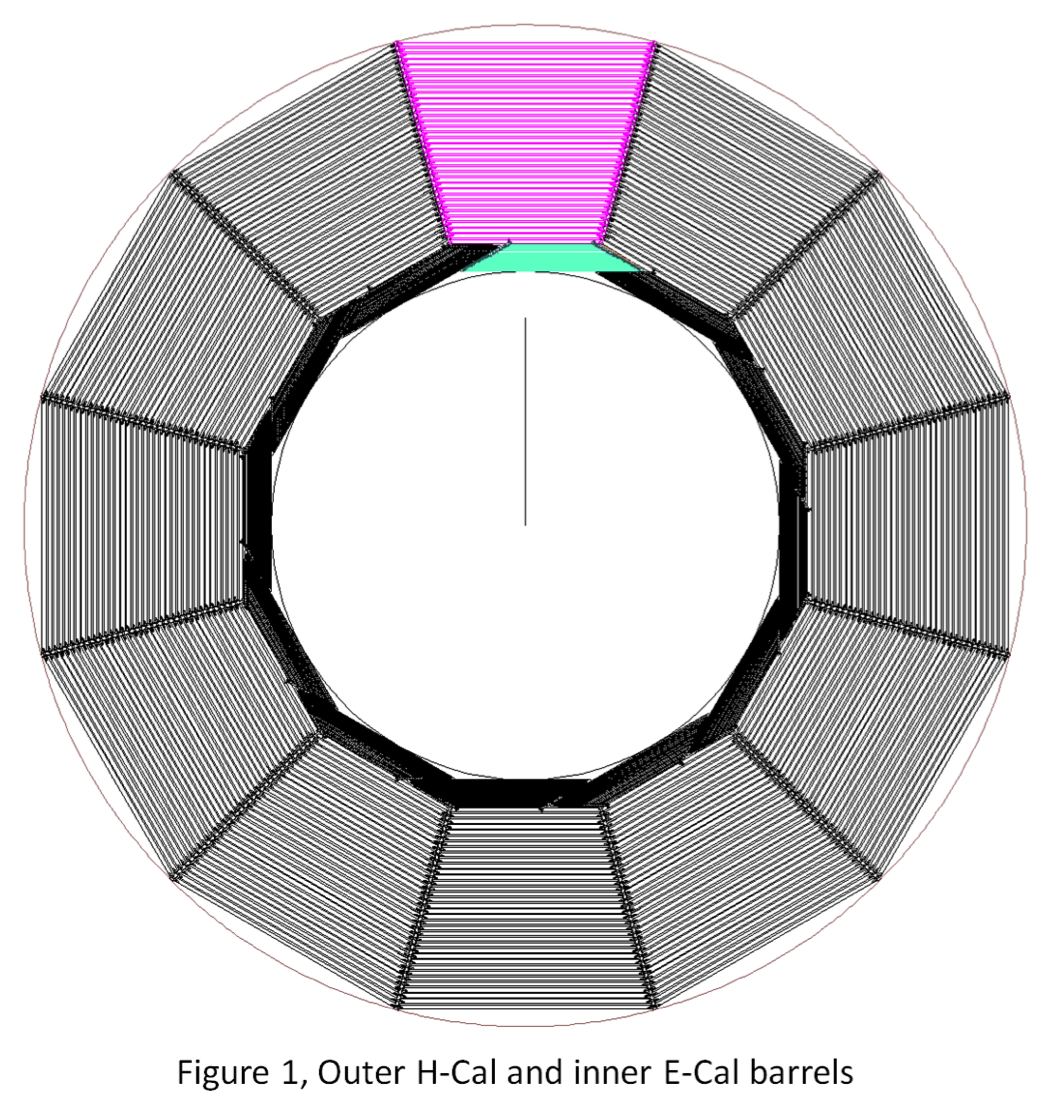
\includegraphics[width=.5\linewidth]{Calorimeter/SiliconTungstenSiD/cross_section}
\end{figure}
\begin{figure}
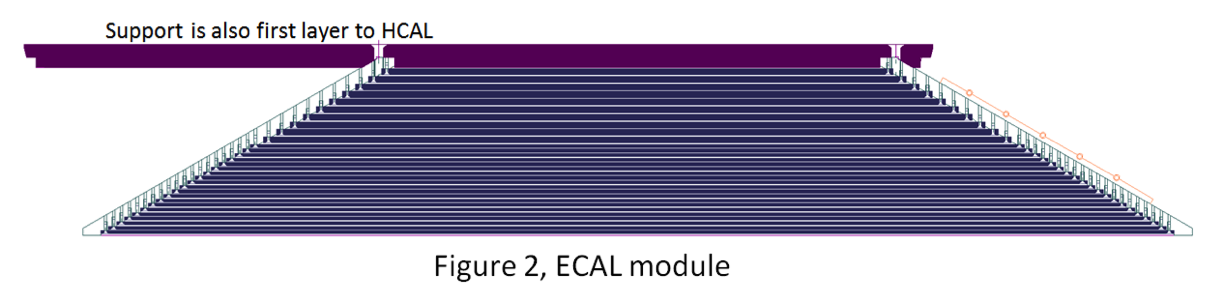
\includegraphics[width=.5\linewidth]{Calorimeter/SiliconTungstenSiD/ecalModule}
\end{figure}
\begin{figure}
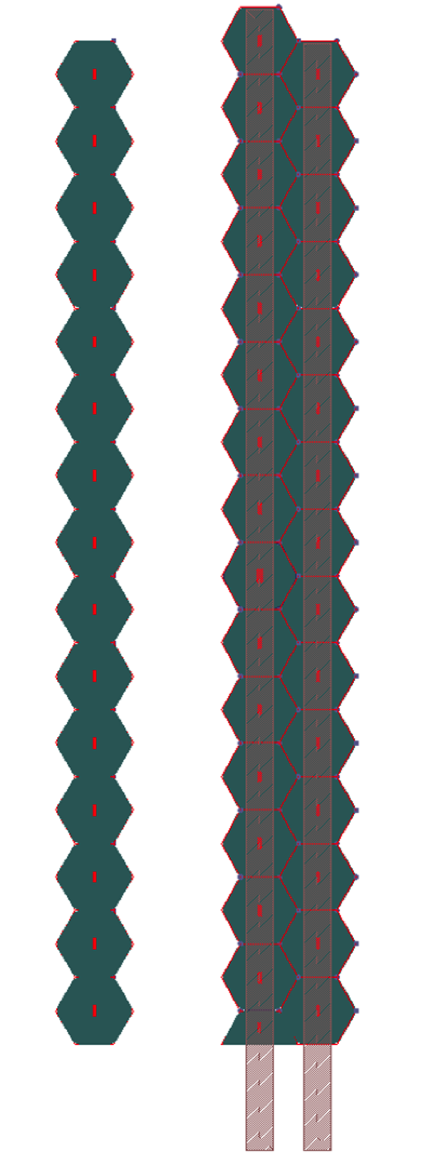
\includegraphics[width=.5\linewidth]{Calorimeter/SiliconTungstenSiD/hexagon}
\end{figure}
\begin{figure}
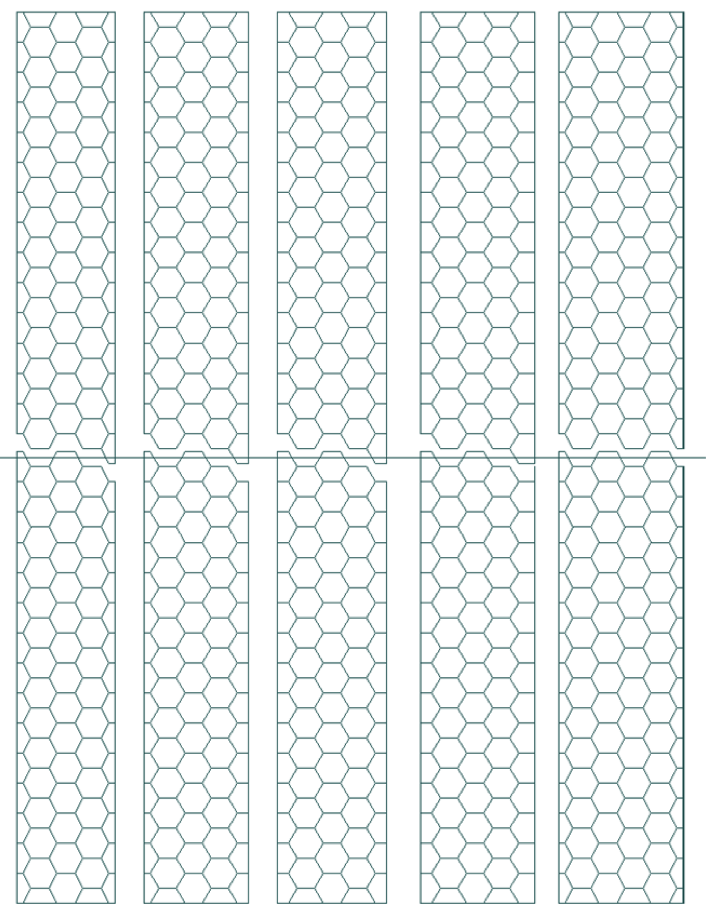
\includegraphics[width=.5\linewidth]{Calorimeter/SiliconTungstenSiD/siliconLayout}
\end{figure}
\begin{figure}
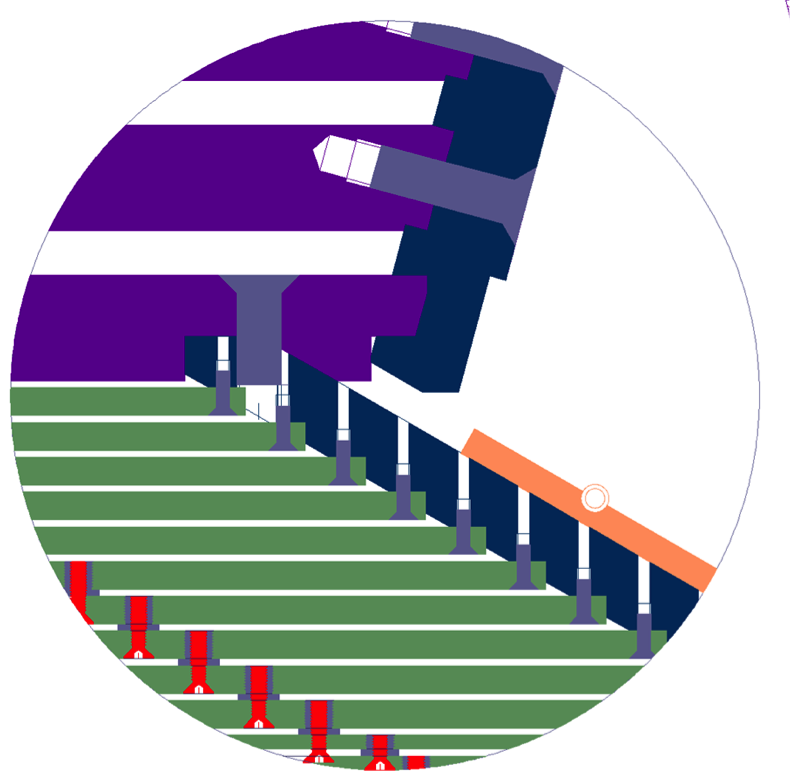
\includegraphics[width=.5\linewidth]{Calorimeter/SiliconTungstenSiD/edgeFasteners}
\end{figure}
\begin{figure}
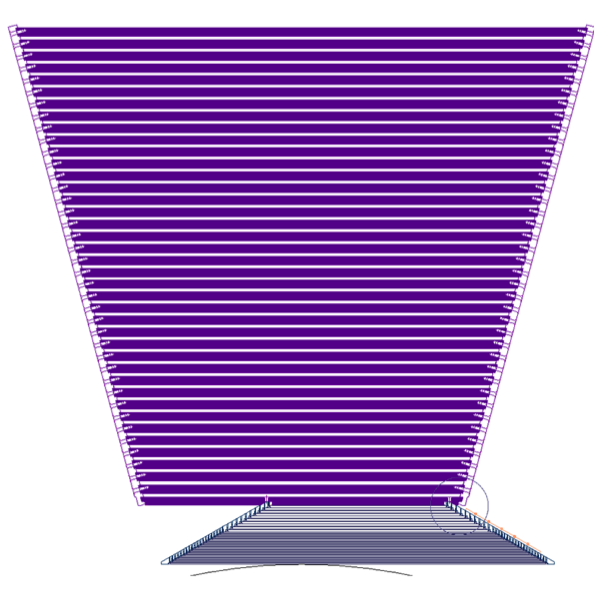
\includegraphics[width=.5\linewidth]{Calorimeter/SiliconTungstenSiD/ecalMounting}
\end{figure}
\begin{figure}
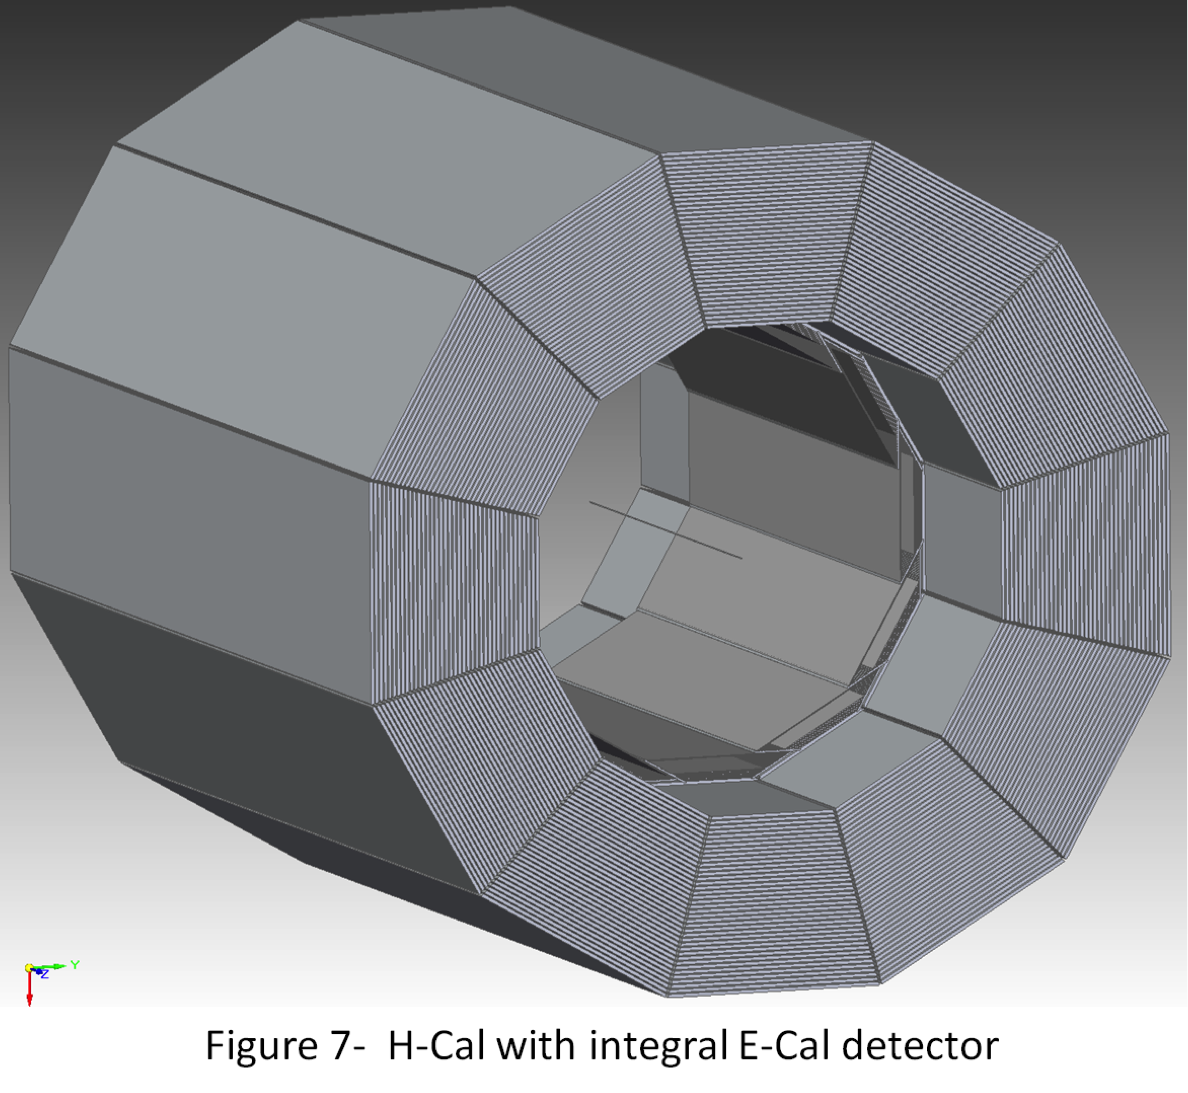
\includegraphics[width=.5\linewidth]{Calorimeter/SiliconTungstenSiD/HCalECal}
\end{figure}
\begin{figure}
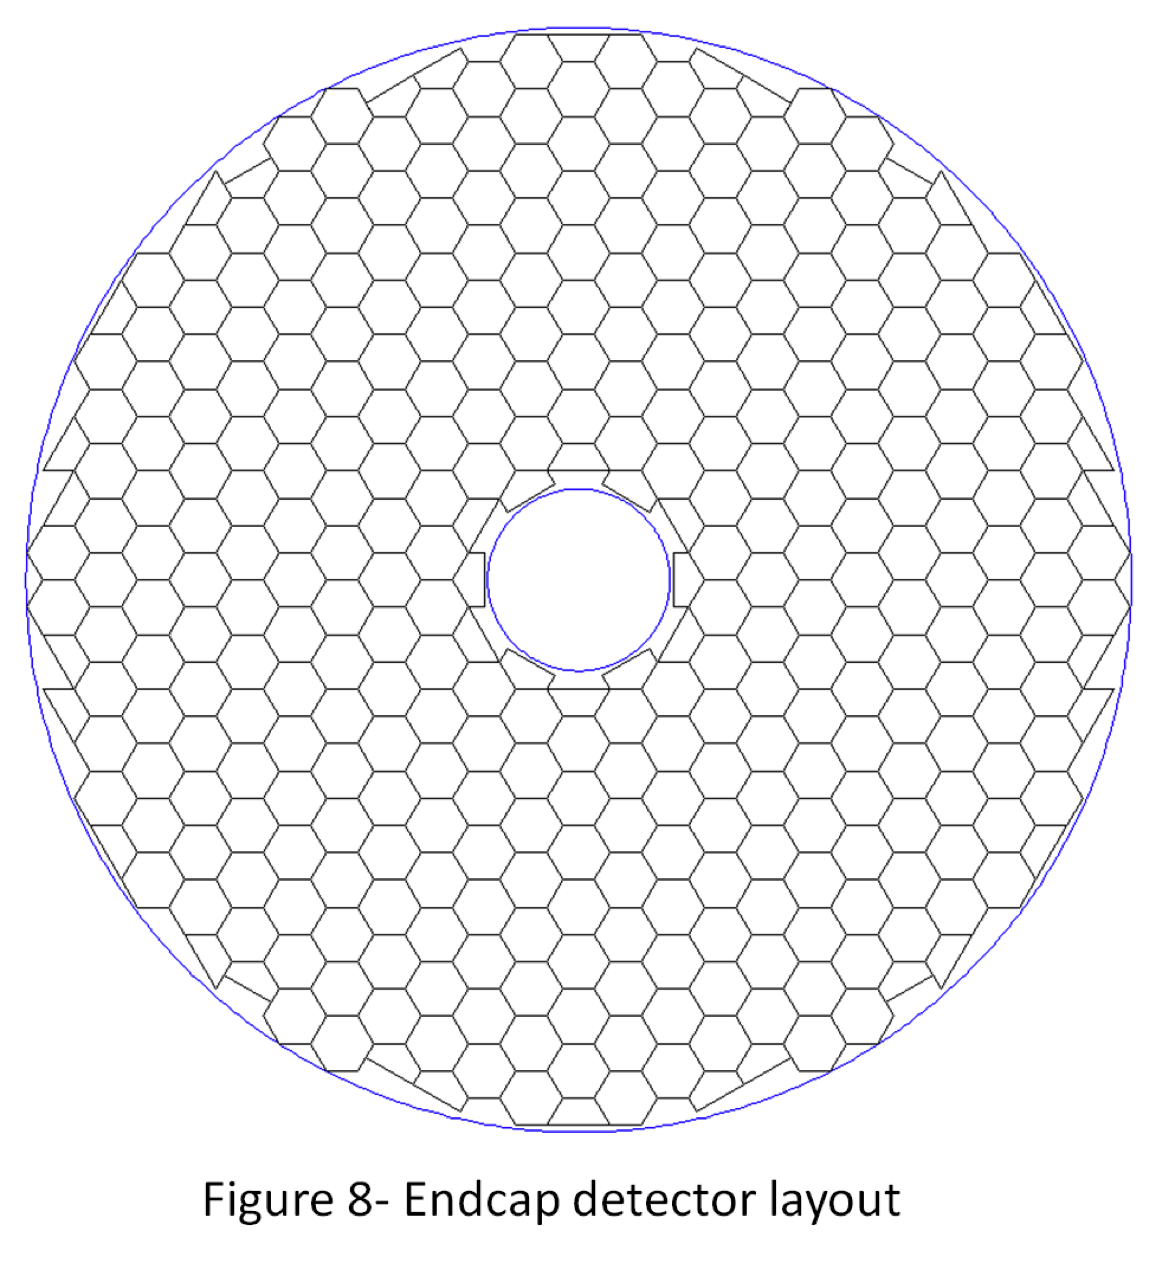
\includegraphics[width=.5\linewidth]{Calorimeter/SiliconTungstenSiD/endcapLayout}
\end{figure}

This note describes the theory of the mechanical aspects of the E-Cal system for SiD.
The E-Cal barrel consists of stacks of tungsten heavy metal plates which are arranged in modules surrounding the beamline. Full cylindrical coverage of the baseline design is attained with twelve modules (see figure 1) occupying a radial envelope from 1265mm to 1409mm. The total barrel length is 3.53m.
Each module uses 20 inner plates which are 2.5mm thick followed by ten 5mm thick plates. Gaps between adjacent plates are 1.25mm and house the silicon detectors with their associated cables (see figure 2). These hexagonal silicon detectors are electrically connected to each other with thin, flexible circuits which are read out on both ends of a module (see figure 3).  Panels of detectors increase in width as they get closer to the beamline. To minimize silicon waste and to maximize coverage, fractions of hexagons complete the panel edges (see figure 4). By cutting the silicon in strategic locations, only a few different silicon shapes may be needed to achieve the 31 different panel widths.
The tungsten plates are connected together on their longitudinal edges as well as in the field of detectors. Space for fasteners in the field is achieved by chamfering the corners of the hexagonal detectors. The field fasteners hold the plates together, provide a uniform 1.25mm standoff height, and assist with inter-plate shear. The fasteners near the edges of the plates close the module profile and lend torsional rigidity to the structure. An FEA simulation of the proposed configuration should be done to properly size the fasteners (see figure 5).The modules, which weigh about 5 tons each, are mounted to stainless plates which are used as the first layer of the next detector system (H-Cal). This first H-Cal plate is unique in that its two longitudinal edges form a guide system to locate the E-Cal to the H-Cal system.  The H-Cal modules are first bolted together to form the H-Cal barrel. Interleaving structural side battens maintain spacing for the H-Cal plates and extend inward to the E-Cal support plates. The inner ends of these battens act in concert as the female portion of the E-Cal guide system. The E-Cal modules are slid into place in the inner H-Cal bore. Extension plates complete the inner H-Cal first layer, since the E-Cal barrel is shorter. H-Cal detector panels are installed after this structure is complete (see figure 7).
Only simple detector layouts have been done for the E-Cal endcaps so far. These layouts show that using full and partial hexagons could yield fairly good coverage with only a few shapes. (see figure 8).
